% !TEX encoding = UTF-8 Unicode
\documentclass[handout]{beamer}
\usepackage[frenchb]{babel}
\usepackage[T1]{fontenc}
\usepackage[utf8]{inputenc}

% functions to plot
\def\func(#1){(#1)*(1-(#1))}
\hypersetup{colorlinks = true,linkcolor = blue,urlcolor  = blue}

\newenvironment{iPar}[1]{\textbf{#1} \begin{itemize}}{\end{itemize}}

\title{Introduction and Rappel Mathématique}
\author{Microéconomie \\ 20851}
\date{}

\begin{document}

\frame{\titlepage}

\section[Outline]{}
\frame{\tableofcontents}

\section{Introduction}
\frame
{
  \frametitle{La microéconomie}
Vos cours de micro jusqu'ici
  \begin{itemize}
  \item<1-> Microéconomie 1-851-07
  \item<2-> Problème et Politiques économiques (PPE), 2-851-07
  \end{itemize}
  \vspace{0.2in}
  La micro est centrale en économie: 
  \begin{itemize}
    \item<3-> La macro s'appuie beaucoup sur la micro (de plus en plus)...
    \item<4-> La micro s'appuie sur la psychologie, la sociologie
    \item<5-> L'intélligence articilielle peut s'alimenter de la micro
  \end{itemize}
}

\begin{frame}{Les microéconomistes et les inégalités}

\begin{figure}
	
\includegraphics[scale=0.35]{justice.png}
	\caption{Voir \href{https://missingprofits.world/}{missingprofits.world} pour une estimation de ce que perd chaque pays vers les paradis fiscaux}
\end{figure}

\end{frame}


\begin{frame}{Les microéconomistes et le climat}

\begin{figure}
	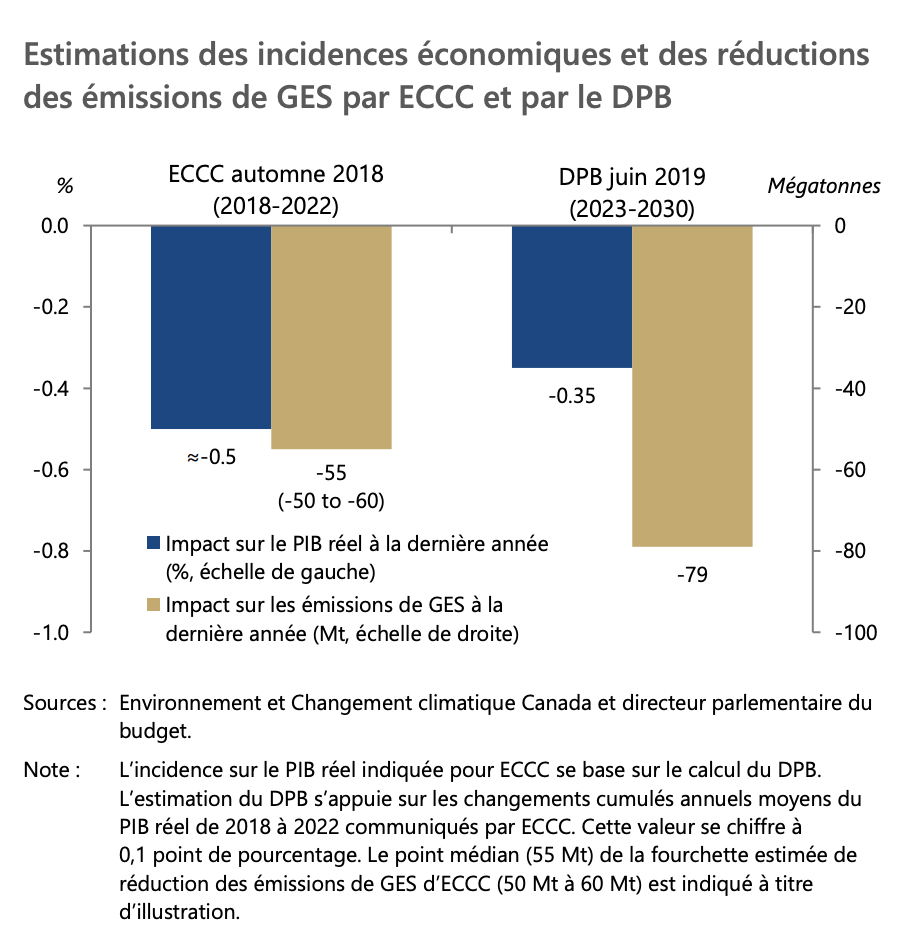
\includegraphics[scale=0.35]{climat.png}
	\caption{Directeur parlementaire du Budget 2019}
\end{figure}

\end{frame}


\begin{frame}{La nouvelle économie}

\begin{figure}
	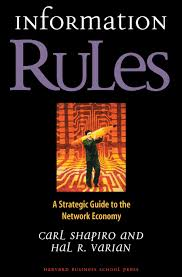
\includegraphics[scale=0.5]{rules.jpeg}
	\caption{Hal Varian est l'économiste en chef chez Google}
\end{figure}

\end{frame}

\begin{frame}{Des microéconomistes chez AirBnB}

\begin{figure}
	
\includegraphics[scale=0.25]{AI.png}
	\caption{The Economist, 2015}
\end{figure}

\end{frame}




\begin{frame}{Les Données: le nerf de la guerre}

Les données sont partout. La théorie aide à en faire du sens:

  \begin{itemize}
  \item<1-> Comprendre les comportements (e.g. tester des théories)
  \item<2-> Quantifier des effets pour porter des jugements positifs et normatifs sur des politiques
  \item<3-> Tarification et optimisation en entreprise
  \item<4-> Un danger est d'exploiter les données sans cadre théorique (voir cet \href{https://www.quantamagazine.org/to-build-truly-intelligent-machines-teach-them-cause-and-effect-20180515/}{article} sur l'intelligence artificielle)
  \end{itemize}

\end{frame}

\section{Structure du cours}

\begin{frame}{Les thèmes couverts}
  \begin{itemize}
  \item<1-> Consommation
  \item<2-> Les marchés et le bien-être
  \item<3-> La production: choix de production
  \item<4-> Les comportements stratégiques
  \item<5-> Les enchères
  \end{itemize}
  
\end{frame}

\begin{frame}{Évaluation}

\begin{itemize}
\item Un devoir individuel (5\%)
\item 3 devoirs en équipe (30\%)
\item Intra (25\%) et final (40\%)
\end{itemize}

\end{frame}

\begin{frame}{Autres remarques}

\begin{itemize}
\item Auxiliaire enseignement: Nicholas Trottier-Lacourse
\item Référence (non-obligatoires) pour cours:
\begin{itemize}
    \item Hal Varian (2015). \textit{Introduction à la microéconomie}, Deboeck
    \item Hal Varian (2008). \textit{Analyse microéconomique}, Deboeck
\end{itemize}
\item Théorie et pratique (programmation sur Google Collab)
\end{itemize}

\end{frame}

\section{Rappel Mathématique}

\begin{frame}{L'analyse marginale et les approximations}

Astuce de l'approximation:

\begin{itemize}\item Fonctions généralement compliquées, fonctions linéaires simples...
\item Localement, on peut faire une approximation de toute fonction "lisse" à $x_0$, pour $x$ près de $x_0$: 
\begin{eqnarray*} 
	f(x) \simeq f(x_0) + \alpha (x-x_0) + ...  
\end{eqnarray*}
\end{itemize}
\textbf{Exercice A}: Montrer graphiquement une approximation de premier ordre.
\end{frame}

\begin{frame}{Lien avec dérivée}
Pour $x$ près de $x_0$
\begin{align*}
&f(x) \simeq f(x_0) + \alpha (x-x_0) \\ \\ \iff & f(x) -f(x_0) \simeq \alpha (x-x_0)\\\\
 \iff & \alpha \simeq \frac{f(x) -f(x_0)}{x-x_0}  \simeq\; f'(x_0) \quad \text{par définition}
\end{align*}
\pause
Alors  \begin{align*}&f(x) \simeq f(x_0) + f'(x_0) (x-x_0) \quad \text{ ou }\\ \\ &f(x) - f(x_0) \simeq f'(x_0) (x-x_0) \quad \text{ ou } \\ \\
&\Delta f \simeq f'(x_0) \Delta x
\end{align*}

\end{frame}

\begin{frame}{Les dérivées de fonctions}

\begin{columns}
\footnotesize
\begin{column}{0.5\textwidth}
   Avec des constantes
   \begin{itemize}
   		\item $f(x) = b + ax$: $f'(x) = a$
		\item $f(x) = \log x$: $f'(x) = \frac{1}{x}$
		\item $f(x) = e^{ax}$: $f'(x) = ae^{ax}$ 
		\item $f(x) = x^a$: $f'(x) = a x^{a-1}$
   \end{itemize}
\end{column}
\begin{column}{0.5\textwidth}  %%<--- here
	Avec des fonctions
	\begin{itemize}
		\item $f(x) = a(x)b(x)$, $f'(x) = a'(x)b(x) + a(x)b'(x)$
		\item $f(x) = \frac{a(x)}{b(x)}$, $f'(x) = \frac{a'(x)b(x) - a(x)b'(x)}{b(x)^2}$
		\item $f(x) = a(b(x))$, $f'(x) = a'(b(x))b'(x)$
		\item $f(x) = a(x) + b(x)$, $f'(x) = a'(x) + b'(x)$. 
	\end{itemize}
\end{column}
\end{columns}
\vspace{0.5in}
\textbf{Exercice B}: Trouvez les dérivées de : $f(x)=\sqrt{x},\frac{x}{1+x},\frac{1}{2}x^2 + 2x-10,(1+\frac{x}{2})^2$.
\end{frame}


\begin{frame}{Approximations d'ordres supérieurs}

On peut pousser l'astuce plus loin
\begin{itemize}
\item Polynome d'ordre 2 assez simple...
\item Alors, on approxime par deuxième ordre
\item Polynome d'ordre $k$ \ldots
\end{itemize}\
\pause
L'astuce porte le nom d'approximation de Taylor. Connectée aux dérivées d'ordres supérieurs d'une fonction:
\begin{eqnarray*}
	f(x) = f(x_0) + f'(x_0)(x-x_0) +\frac{1}{2}f''(x_0)(x-x_0)^2 + \ldots 
\end{eqnarray*}
On dénote $f'(x), f''(x)$ ou $\frac{d f}{d x},\frac{d}{d x}(\frac{d f}{d x}) = \frac{d^2 f}{d x^2} $.
\end{frame}

\begin{frame}{Concavité et Convexité des fonctions}

Une fonction est convexe si pour tous points $(x_1,x_2)$ et tout $\lambda>0,0<\lambda<1$: 
\begin{align*}
f(\lambda x_1 + (1-\lambda) x_2) \leq \lambda f(x_1) + (1-\lambda)f(x_2)
\end{align*}

et concave si l'inverse est vrai. On dit strictement si les inégalités sont strictes. 

\end{frame}



\begin{frame}{Approximation et maximization (sans contrainte)}

Considérons l'approximation de premier ordre:
\begin{eqnarray}
 f(x_0+\Delta x) \simeq f(x_0)+ f'(x_0)\Delta x 
\end{eqnarray}

Observons que:
\begin{itemize}
\item Si $f'(x_0)>0$  un petit changement $\Delta x>0$ augmente $f$
\item Si $f'(x_0) <0$ un petit changement $\Delta x <0$ augmente $f$
\item Si $x_0$  est la solution de  $\max_x f(x)$, il faut que $f'(x_0) =0$
\end{itemize} 
\end{frame}

\begin{frame}{Maximisation sans contrainte}

Considérons l'approximation de deuxième ordre:
\begin{eqnarray}
 f(x_0+\Delta x) \simeq f(x_0) + f'(x_0)\Delta x +\frac{1}{2}f''(x_0)\Delta x ^2  
\end{eqnarray}

Pour un maximum (local), il faut que $f'(x_0)=0$ (CPO) et $f''(x_0)<0$ (CDO). 
Observons que:
\begin{itemize}
\item Si $f'(x_0) = 0$ mais $f''(x_0)>0$, alors $f(x_0+\Delta x) > f(x_0)$. 
\item f'(x) doit être positif quand $\Delta x <0$ et négatif quand $\Delta x>0$. 
\end{itemize}

\textbf{Exercice C}: Montrer graphiquement l'optimum d'une fonction concave.
\end{frame}


\begin{frame}{Théorème de l'enveloppe}

Considérons la fonction $f(x,p)$ où $p$ est hors de contrôle (exogène). On dénote:

\begin{eqnarray*}
 V(p) = \max_x f(x,p) , \quad x^*(p) = \arg \max_x f(x,p)
\end{eqnarray*}

On a que $V(p) = f(x^*(p),p)$. Ainsi, 

\begin{eqnarray}
V'(p) = f'_x(x^*(p),p)x^{*'}(p) + f'_p(x^*(p),p)
\end{eqnarray}
Or, puisque $x^*(p)$ maximise $f(x,p)$, $f'_x(x^*(p),p) = 0$ par définition. Ainsi, $V'(p) = f'_p(x^*(p),p)$.  

\textbf{Exercice D}: Démontrer la valeur de cette approximation pour la fonction $V(p) = (10 - p\frac{x}{2})x$. 
\end{frame}

\begin{frame}{Maximisation avec contrainte}

Considérons le problème: 
\begin{eqnarray*}
	\max_x \{f(x):x \leq x_0\}
\end{eqnarray*}

Un maximum est atteint si $f'(x)=0$ (nécessaire). Or si $f'(x)>0 $ pour tout $ x \leq x_0$, le maximum contraint est $x_0$. Relacher la contrainte marginalement de $x_0$ fait gagner $f'(x_0)\Delta x$.  


\end{frame}

\begin{frame}{Plusieurs variables}

Supposons la fonction $f(x,y)$. La dérivée partielle se fait en gardant fixe (ou exogène) les autres variables: $f'_x(x,y) = \frac{\partial f(x,y)}{\partial x}$.

\end{frame}

\begin{frame}{La différentielle totale}

Les combinaisons de $x,y$ tels que $f(x,y) = \overline{f}$) peuvent être trouvées par solution directe, $y=g(x,\overline{f})$. Mais on peut décrire ces combinaisons plus facilement en utilisant la différentielle totale (une approximation linéaire): 

On peut décrire la forme de cette fonction par: 

\begin{eqnarray*}
df(x,y) = f'_x(x,y)dx + f'_y(x,y)dy
\end{eqnarray*}

Si on pose $df(x,y)=0$, 

\begin{eqnarray*}
\frac{dy}{dx}\Bigr|_{df=0} = -\frac{f'_x(x,y)}{f'_y(x,y)}
\end{eqnarray*}
 
\textbf{Exercice E}: Trouvez $\frac{dy}{dx}\Bigr|_{df=0}$ par différentielle totale pour $f(x,y)=\log(xy)$. 
\end{frame}


\begin{frame}{Homogénéité des fonctions}

Une fonction est homogène de degré $r$ si pour tout $\lambda>0$, 
\begin{align*}
f(\lambda x_1, \lambda x_2, ... \lambda x_n) = \lambda^r f(x_1,x_2,...,x_n)
\end{align*}

Si une fonction est homogène de degré $r$, alors ceci est aussi vrai (théorème d'Euler):
\begin{align*}
r f(x_1,x_2,...,x_n) = \sum_{i=1}^n \frac{\partial f}{\partial x_i}x_i
\end{align*}

\textbf{Exercice F}: Trouvez le degré d'homogénéité de la fonction $f(x,y)=x^\alpha y^\beta$ des deux façons.
\end{frame}

\begin{frame}{Approximation et Maximum}

\begin{eqnarray*}
f(x,y) \simeq f(x_0,y_0) + f'_x(x_0,y_0)(x-x_0) + f'_y(x_0,y_0)(y-y_0)  \\
	+\frac{1}{2}f''_{xx}(x_0,y_0)(x-x_0)^2  + \frac{1}{2}f''_{yy}(x_0,y_0)(y-y_0)^2 + \\
	+f''_{xy}(x_0,y_0)(x-x_0)(y-y_0) 
\end{eqnarray*}

Condition pour un maximum: 
\begin{itemize}
\item Nécessaire: $f'_x(x,y)=0, f'_y(x,y)=0$
\item Suffisante: $\frac{1}{2}f''_{xx}(x_0,y_0)(x-x_0)^2  + \frac{1}{2}f''_{yy}(x_0,y_0)(y-y_0)^2 +f''_{xy}(x_0,y_0)(x-x_0)(y-y_0)<0$ 
\end{itemize}

\end{frame}

\begin{frame}{Maximisation avec contrainte}

Approche directe. Quand le problème prend la forme:

\begin{eqnarray}
\max_{x,y} \{ f(x,y): g(x,y)=m\}
\end{eqnarray}

Et qu'on peut inverser $g(x,y)=m$ tel que $y=q(x,m)$, alors la solution du problème contraint pour $x$ est la même que celui de :

\begin{eqnarray}
\max_{x} \{ f(x,q(x))\}
\end{eqnarray}

La CPO est $f'_x(x,q(x,m)) + f'_y(x,q(x,m))q'(x,m) = 0$. On peut résoudre pour $x^*$ et utiliser $y=q(x)$ pour trouver $y^*$. Facile, mais quand plus de 2 variables?

\textbf{Exercice G}: Maximiser la fonction $f(x,y) = \log x + \log y$ sous la contrainte $x+y \le m$.
\end{frame}

\begin{frame}{Le Lagrangien}

La méthode de Lagrange consiste à résoudre pour $(x,y)$, 

\begin{eqnarray}
f'_x(x,y) -  \lambda g'_x(x,y) = 0 \\
f'_y(x,y) -  \lambda g'_y(x,y) = 0 \\
g(x,y) = m
\end{eqnarray} 

Ce sont les CPO du lagrangien: 
\begin{eqnarray}
	\max_{x,y,\lambda} f(x,y) - \lambda (g(x,y)-m)
\end{eqnarray} 

\textbf{Exercice H}: Maximiser la fonction $f(x,y) = \log x + \log y$ sous la contrainte $x+y \le m$ par la méthode du Lagrangien.
\end{frame}

\begin{frame}{L'interprétation du multiplicateur}

La valeur de $\lambda$ n'est pas nécessaire pour résoudre les valeurs optimales de $x$ et $y$. Mais elle a une  interprétation.

Par le théorème de l'enveloppe, si $$V(m) = \max_{x,y,\lambda} f(x,y) - \lambda (g(x,y)-m)$$

alors $V'(m) = \lambda$. 
\vspace{0.5in}

\textbf{Exercice I}: Démontrer dans le problème précédent qu'une augmentation marginale de $m$ sur le maximum est bien égale à $\lambda$. 
\end{frame}

\end{document}